\chapter{Déploiement}

\section{Introduction}

Ce chapitre présente le déploiement de l'application de détection de textes générés
par intelligence artificielle. L'application est composée d'un backend FastAPI et
d'un frontend React, tous deux déployés sur la plateforme Render.

\section{Technologies utilisées}

\subsection{FastAPI}

FastAPI est un framework Python utilisé pour développer l'API REST de l'application.
Il expose deux routes principales décrites dans le tableau \ref{tab:api_routes}.

\begin{table}[H]
\centering
\renewcommand{\arraystretch}{1.4}
\begin{tabular}{|c|c|p{7cm}|}
\hline
\textbf{Méthode} & \textbf{Route} & \textbf{Description} \\
\hline
GET  & \texttt{/}        & Vérification du statut de l'API \\
\hline
POST & \texttt{/predict} & Classification d'un texte soumis \\
\hline
\end{tabular}
\caption{Routes de l'API FastAPI}
\label{tab:api_routes}
\end{table}

\subsection{React et Vite}

Le frontend est développé avec React et Vite. Il permet à l'utilisateur de saisir
un texte, de lancer l'analyse et de consulter le résultat de la classification
ainsi que l'historique des analyses.

\subsection{Render}

Render est une plateforme cloud gratuite permettant d'héberger des applications web.
Elle a été choisie pour sa simplicité de déploiement depuis GitHub, son support natif
de Python et de Node.js, et la génération automatique d'un certificat HTTPS.

\subsection{Git et GitHub}

Git est utilisé pour le versionnement du code source et GitHub comme dépôt distant.
Render se connecte au dépôt GitHub et déclenche automatiquement un nouveau
déploiement à chaque push.

\section{Déploiement sur Render}

\subsection{Étapes de déploiement}

Le déploiement du backend et du frontend s'effectue en suivant les étapes suivantes :

\begin{enumerate}
    \item Le code source complet (backend et frontend) est poussé vers le dépôt GitHub.

    \item Un premier Web Service est créé sur Render pour le \textbf{backend} avec
    les paramètres : \textit{Root Directory} = \texttt{backend},
    \textit{Build Command} = \texttt{pip install -r requirements.txt},
    \textit{Start Command} = \texttt{uvicorn main:app -{}-host 0.0.0.0 -{}-port \$PORT}.

    \item Un second Web Service est créé sur Render pour le \textbf{frontend} avec
    les paramètres : \textit{Root Directory} = \texttt{frontend},
    \textit{Build Command} = \texttt{npm install \&\& npm run build},
    \textit{Publish Directory} = \texttt{dist}.

    \item Render installe automatiquement les dépendances, compile les fichiers
    et démarre les deux services.

    \item L'URL publique du backend est renseignée dans le frontend pour
    que les appels API pointent vers le service déployé.
\end{enumerate}

\subsection{Résultat}

Une fois déployés, les deux services sont accessibles aux adresses suivantes :

\begin{itemize}
    \item \textbf{Frontend} : \url{https://ai-text-detector.onrender.com}
    \item \textbf{API} : \url{https://ai-text-detector-api.onrender.com}
    \item \textbf{Documentation} : \url{https://ai-text-detector-api.onrender.com/docs}
\end{itemize}

\section{Tâches réalisées}
Les figures suivantes illustrent les deux cas de classification de l'application.
La figure \ref{fig:screenshot_human} montre un texte classifié comme humain et
la figure \ref{fig:screenshot_ai} montre un texte classifié comme généré par IA.

\vspace{0.3cm}

\begin{figure}[H]
    \centering
    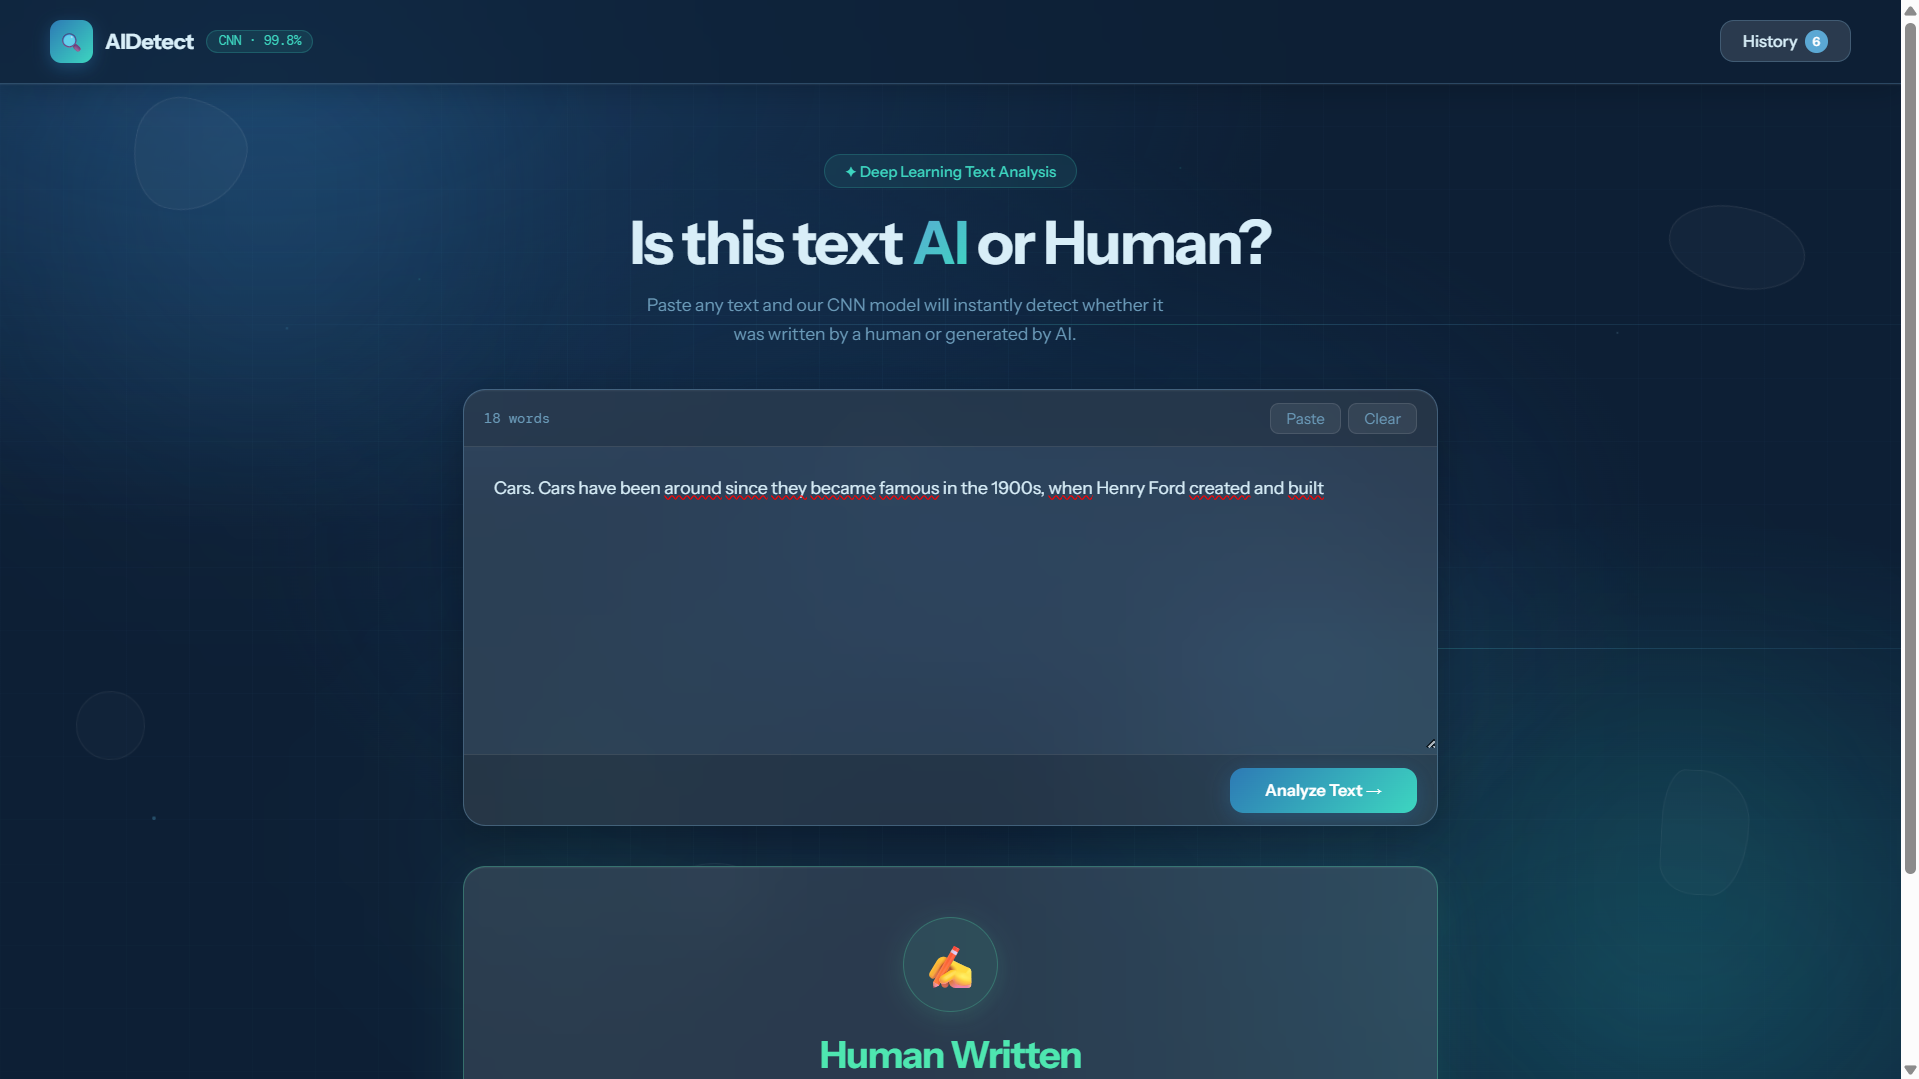
\includegraphics[width=0.80\linewidth]{Screenshot 2026-03-14 140009.png}
    \caption{Résultat \textit{Human Written} — texte classifié comme rédigé par un humain.}
    \label{fig:screenshot_human}
\end{figure}

\vspace{0.5cm}

\begin{figure}[H]
    \centering
    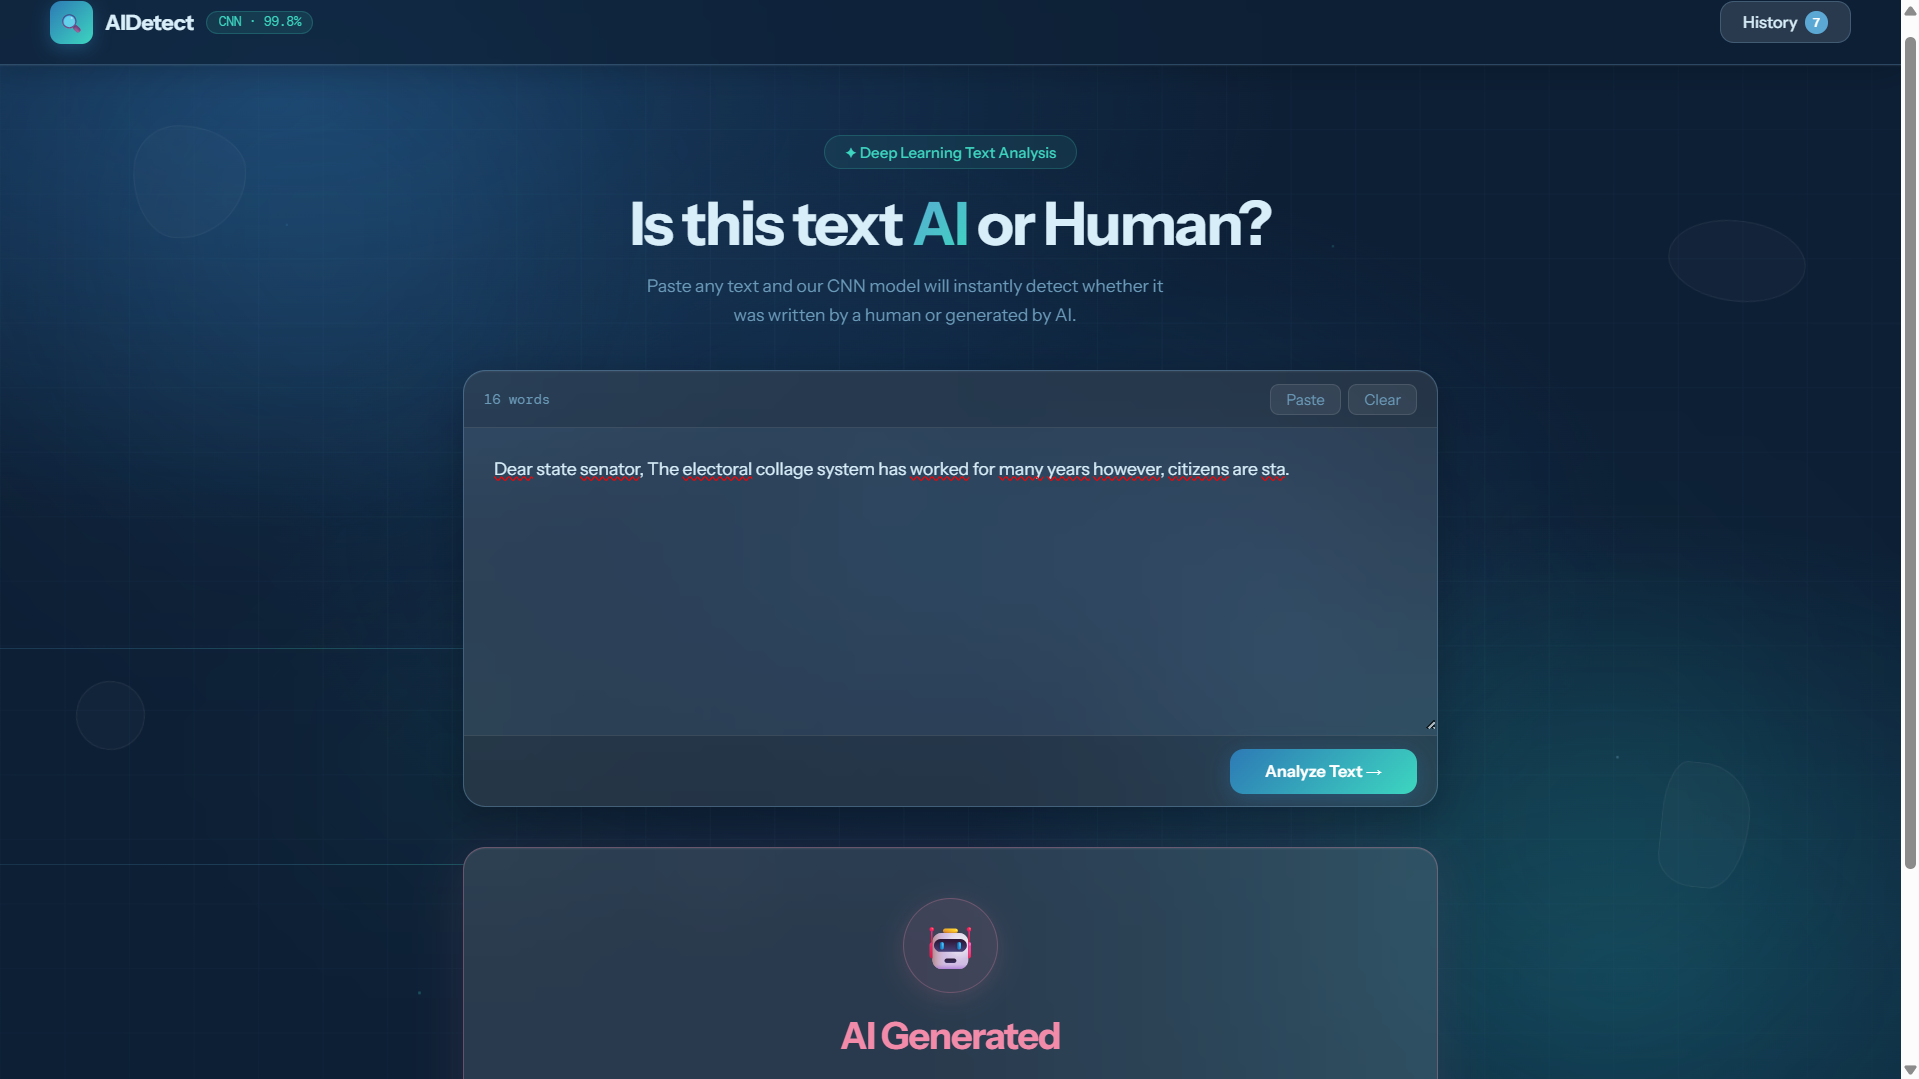
\includegraphics[width=0.80\linewidth]{Screenshot 2026-03-14 140034.png}
    \caption{Résultat \textit{AI Generated} — texte classifié comme généré par une IA.}
    \label{fig:screenshot_ai}
\end{figure}

\section{Conclusion}

Ce chapitre a présenté le déploiement complet de l'application sur la plateforme Render,
aussi bien le backend FastAPI que le frontend React. Cette architecture entièrement
hébergée en ligne permet une utilisation accessible depuis n'importe quel navigateur,
sans nécessiter d'installation locale. La synchronisation entre GitHub et Render assure
un redéploiement automatique à chaque mise à jour du code source.